\hoofdstuk{Defining the context}
The goal of this chapter is to define the context of the main research question.

\indent \emph{"How to develop a cross-platform mobile application while retaining the native look-and-feel?"}

\noindent Accordingly this chapter will define:
\begin{itemize}
\item the scope of \emph{cross-platform}
\item the concept of the \emph{native look-and-feel}
\end{itemize}

\paragraaf{Cross-platform}
This section will define the scope of \emph{cross-platform}. This will be done in two parts, first term platform will be defined after which will determined which platforms fall within the scope.

\subparagraaf{Platforms}
In order to determine which platforms should be supported for mobile development the following criteria have been provided by Lunatech:

\begin{enumerate}	
\item \emph{Platform type}\\
The platform has to be mobile, equipped with a touchscreen and support 3rd party applications. %Only smartphones will be targetted for development.
\item \emph{Platform marketshare}\\
The platform should have 10\% market share in the european continent.
\item \emph{Platform marketshare trend}\\
The market share trend from the past 6 months should not depict a trend directed below the set threshold of 10\% within the next 6 months.
\end{enumerate}

The platform type criteria is based on Lunatech's requirement to support smartphones and tablet computers. A smartphone can be defined as a smart phone is a next-generation, multifunctional cell phone that provides voice communication and text-messaging capabilities and facilitates data processing as well as enhanced wireless connectivity.\cite{Ni2006} Tablet computers, commonly referred to as tablet PCs, are wireless portable personal computers that utilize a touchscreen to access or process information.\cite{Leigh2011} The platform market share is the percentage per platform representing its share of the platforms market. Platform market share trend defined as the general course or prevailing tendency of the platforms market share. %TODO spellcheck. TODO: bron toevoegen http://dictionary.reference.com/browse/trend


%The smartphone only criteria implies that it is not a requirement to support support tablets and other mobile devices. This has significant influence on the marketshare criteria because it eliminates marketshare statistics based on operatingsystems, instead specific version details to be be included. %For instance this means that statistics which were harvested based on useragent strings have to be specifically scanned for \emph{iPhone} rather than \emph{Safai Mobile}.

\subparagraaf{Platform marketshares \& trend}
Platforms included in the cross-platform scope need to have a 10\% in share in the european smartphone market. 

There are several sources which provide statistical data over mobile platform market share. One of these is \emph{Net Market Share}. Net Market Share defines itself as the standard for tracking key internet technology usage market share. This means their statistical data is usage based, because it is aggregated from tracking users on the internet. Net market share aggregates its data from over 40,000 websites with approximately 160 million visitors per month.\cite{NetApplications2012}


An alternate source for market share data is \emph{Gartner}. Gartner describes itself as being the world's leading information technology research and advisory company.\cite{Gartner2012} In an annual publication Gartner publishes a smartphone market share report. In contrast to Net Market Share this report has been based on manufacture unit sales data. Although very accurate, it does not reflect real usage nor is it an up to date source, i.e. the latest publication dates from august 2011.\cite{Pettey2011} Therefore Net Market Share is favorable over Gartner.


\begin{centering}
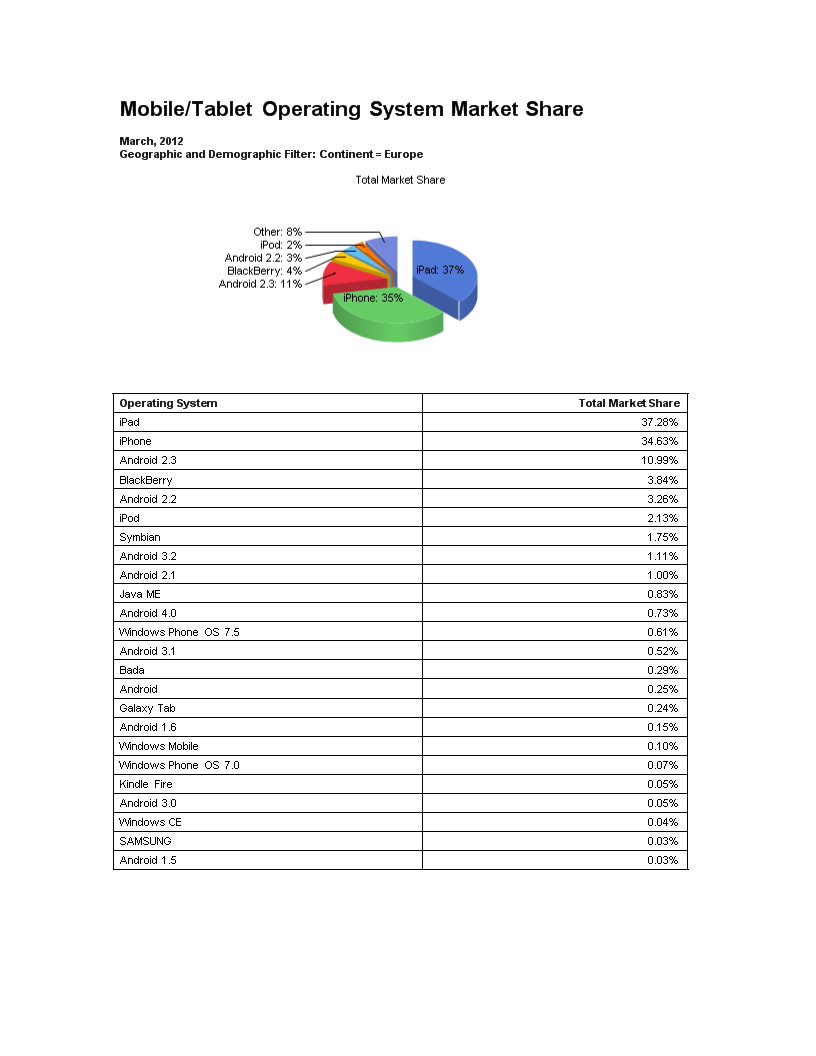
\includegraphics[scale=0.5]{images/netmarketshare_march2012.png}\\
\end{centering}

% \begin{tabel}{|>\R p{\Procent{25}} | >\R p{\Procent{25}} |}{vbx}{Marketshare in the european continent as of march 2012\cite{Netmarketshare2012}}
% \hline
% \bf{Operating System} & \bf{Total \% Market Share}\\
% \hline \hline
% iOS & 74.04\\
% Android & 18.36\\
% BlackBerry & 3.84\\
% Symbian & 1.75\\
% Java ME & 0.83\\
% Windows Phone & 0.68\\
% Bada & 0.29\\
% Windows Mobile & 0.14\\
% Kindle & 0.05\\
% Samsung & 0.03\\
% LG & 0.01\\
% ZTE & 0.00\\
% Palm & 0.00\\
% \hline
% \end{tabel}

% \begin{centering}
% 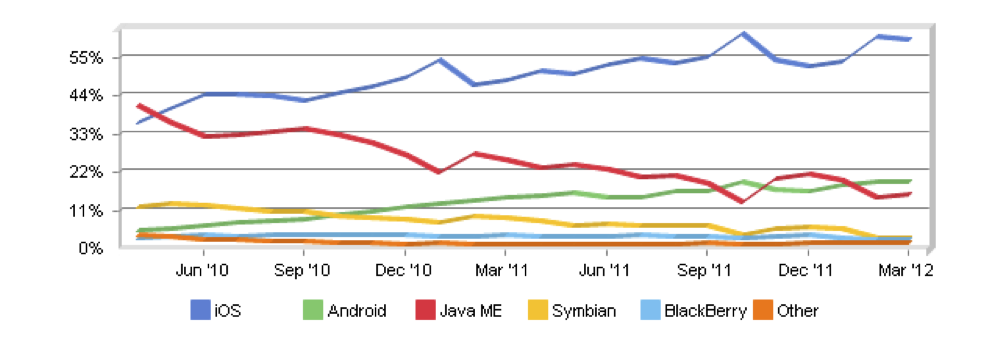
\includegraphics[scale=0.6]{images/marketsharetrendsApril10Tomay12.png}\\{World wide mobile OS Marketshare trends, April 2010 up to may 2012}\\
% \end{centering}

\begin{tabel}{|>\R p{\Procent{25}} | >\R p{\Procent{25}} |>\R p{\Procent{25}} |}{vbx}{Market share in the european continent as of October 2011 and March 2012\cite{Netmarketshare2012}}
\hline
\bf{Operating System} & \bf{Market Share in October 2011} & \bf{Market Share in March 2012}\\
\hline \hline
iOS & 75.78 & 74.04\\
Android & 16.14 & 18.36\\
BlackBerry & 3.56 & 3.84\\
Symbian & 2.69 & 1.75\\
Java ME & 0.87 & 0.83\\
Windows Phone & 0.27 & 0.68\\
Bada & 0.35 & 0.29\\
Windows Mobile & 0.27 & 0.14\\
Kindle & 0.00 & 0.05\\
Samsung & 0.06 & 0.03\\
LG & 0.01 & 0.01\\
\hline
\end{tabel}

iOS and Android both cover over 10 \% of the market, together they are good for 92.40 \% of the total mobile market as of march 2012 in the european continent.


% dit lijkt weg te kunnen:
% There are serveral sources for statistics relating to mobile platform marketshare. Although each based on their own source for gathering statisical data, there are generally 3 ways to collect such data:
% \begin{enumerate}
% \item \emph{Interview based}\\
% A market survey based on data gathered from (public) interviews.
% \item \emph{Sales based}\\
% A market survey based on the calculations from manufactorer sales data.
% \item \emph{Usage probing}\\
% A market survey where the device specific properties are measured to collect data.
% \end{enumerate}

% An interview based method of gathering does relies on the following algorithm provide an realistic image:

% A sales based does not j therefor i. Therefor method based on usage probing is favorable.
% Netmarketshare is a company which provides statistcs based on the usage probing method. It does this by collecting data from the useragent string. This is a piece of information a browser (and thus the device)\footnote{Although the useragent string is manipulatable we neglect this possibility} identifies itself with.



\subparagraaf{Platform versions}
In order to determine which versions per platform will be supported Lunatech has stated that a version must have at least a 10\% user share of the platform. 

\noindent For Android this means the versions:
\begin{itemize}
\item 2.2 - \emph{Froyo} (19.1\%)
\item 2.3.3 to 2.3.7 - \emph{Gingerbread} (64.6\%)
\end{itemize}
This statement is based on data gathered by the number of Android devices that have accessed Google Play within a 14-day period ending on the data collection date noted below.
\begin{centering}
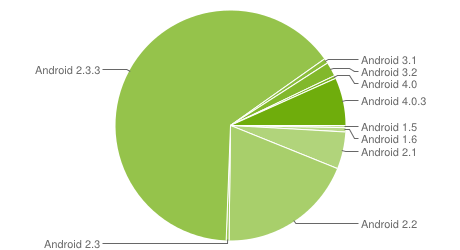
\includegraphics[scale=0.35]{images/androidversionchart.png}\\{Android platform version distribution, as of June 1st, 2012.\cite{GoogleAndroid2012}}\\
\end{centering}

\noindent For iOS this includes the versions:
\begin{itemize}
\item 4.3 (15.0\%)
\item 5.1 (84.0\%)
\end{itemize}
\begin{centering}
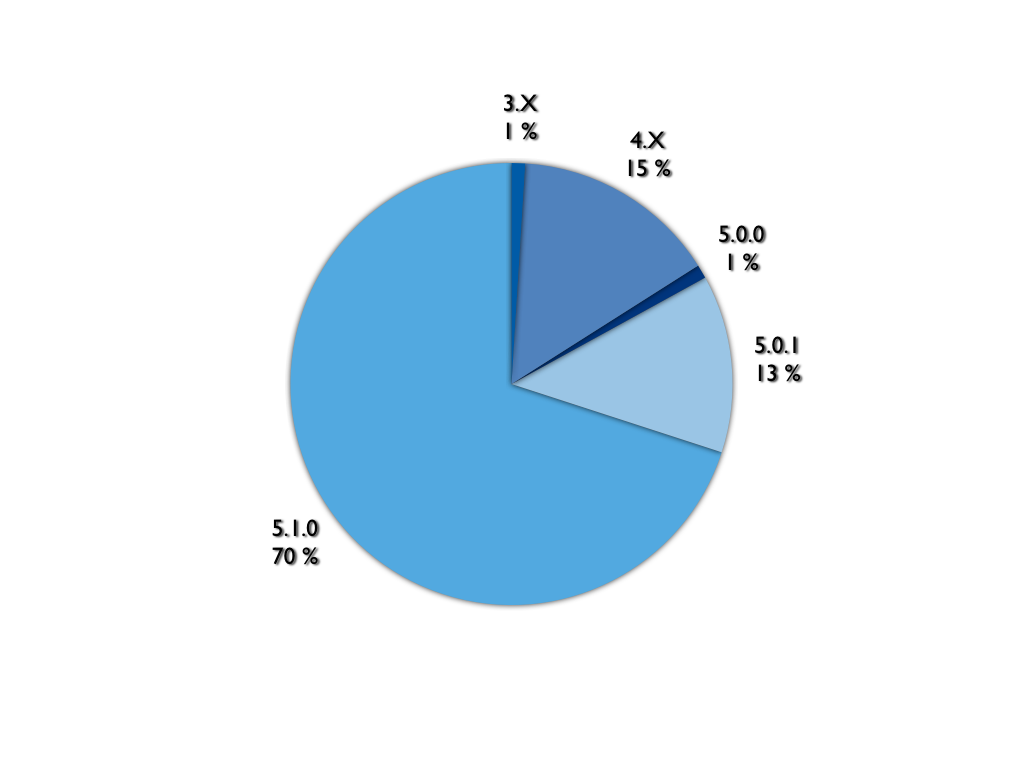
\includegraphics[scale=0.35]{images/iosversionchart.png}\\{iOS platform version distribution, as of May 26th, 2012.\cite{Sylvain2012}}\\
\end{centering}



\subparagraaf{Conclusion}
Apple iOS and Google Android both adhere to the criteria set by Lunatech and will be included in the scope of cross-platform. In conclusion \emph{cross-platform} support is defined as compatible to run on iOS 4.3 or greater and Android 2.2 or greater.


\paragraaf{Native mobile applications}
This paragraph will define the paradigm of \emph{native look-and-feel}. 

A native application is an application inherent to the platform for which it was built using techniques proprietary to the platform. For example, an iOS application is native when written in Objective-C and an Android application is written in Java.  Native applications are typically fast and can access the device's native API's.

\subparagraaf{The native look-and-feel}
When written in the native framework for a platform a mobile application receives access to the available public libraries of the platform. These libraries include those which provide the developer with a pre-fabricated set of user interface components. These can be seen as the building blocks for the graphical user interface on that platform. When used, the general style of the mobile application gains constancy to the overall user interface design of the platforms operating system. This gives an application its native look, which in turn participates to the \emph{native feel}.

%with a feeling of recognition when using the application, userinterface elements work as they expected based upon experience with using the operating system.
%todo: add some notes about the Human Interface Guidelines.

The \emph{native feel} of a mobile application can be defined as the speed in which the user interface elements, the responsiveness of user interface elements to touch events, and smoothness of the animation in which the user interface elements are moved. A native mobile application has the advantage of hardware acceleration. This means its code has been precompiled and directly executed by the device CPU, rather than having to be interpreted by the device's browser. As a result of this the user interface elements are rendered faster and it \emph{feels} smooth.


\paragraaf{Alternative mobile application types}
\subparagraaf{Web applications}
A mobile web application is an application developed with web technologies such as JavaScript and HTML with CSS. It is in fact nothing more than a website designed to fit on a mobile device's display, often they resemble the style of a native application rather than a traditional website. These applications are built with a JavaScript library to add support for scrolling and handling events. Touch events are handled via user interface elements provided by the library. Examples of these libraries include jQtouch, SenchaTouch

% todo: screenshots/links neerzetten.

\subparagraaf{Hybrid applications}
A hybrid application in mobile development refers to an application which use a native shell wrapped around web app. There are generally two forms of native shells, the first is a \emph{webview} and the second a native framework which exposes an JavaScript API to provide the web application access to otherwise native API's.
%TODO framework example.

{\bf Webview-based hybrid applications}\\
A web-view based hybrid application is a web based mobile application wrapped in a web-view. A web-view is a view or element which acts like a browser would, e.g. it is able to render HTML and run javascript.  It is readily available in the native libraries. The advantage of a web-view based hybrid application over an normal web application is that it can be published via the devices native application publishing platforms, i.e. a web-view based hybrid application targeted for the iPhone can be placed in the Apple Appstore. 

Worklight is an example of a framework which can be used to develop web-view based hybrid applications.

{\bf Framework hybrid applications}\\
A Framework based hybrid application is a web-view based application built upon a framework which provides an API to allow the application access to otherwise native API's. The framework is written in the platforms native programming language making it possible to access the native API, such as reading contact list, composing of text messages, full access to the location API, etc.

PhoneGap is an example of a framework which can be used to develop mixed hybrid applications.

\paragraaf{Comparison}
Web applications are quick and cheap to develop. Written entirely in HTML, CSS and JavaScript. Executed by the mobile
browser and therefore cross - platform by default, but less powerful than native apps.
 
Hybrid Applications (Web), the app's source code consists of web code executed within a native wrapper that is provided by a framework.
 
Hybrid Applications (Mix), the developer augments the web code with a Javascript API to create unique features and
access native APIs that are not yet available via the browser, such as AR, NFC and others.
 
Native Application are platform-specific. Requires unique expertise and knowledge. Pricey and time consuming to develop but
 delivers the highest user experience of all approaches.

\begin{centering}
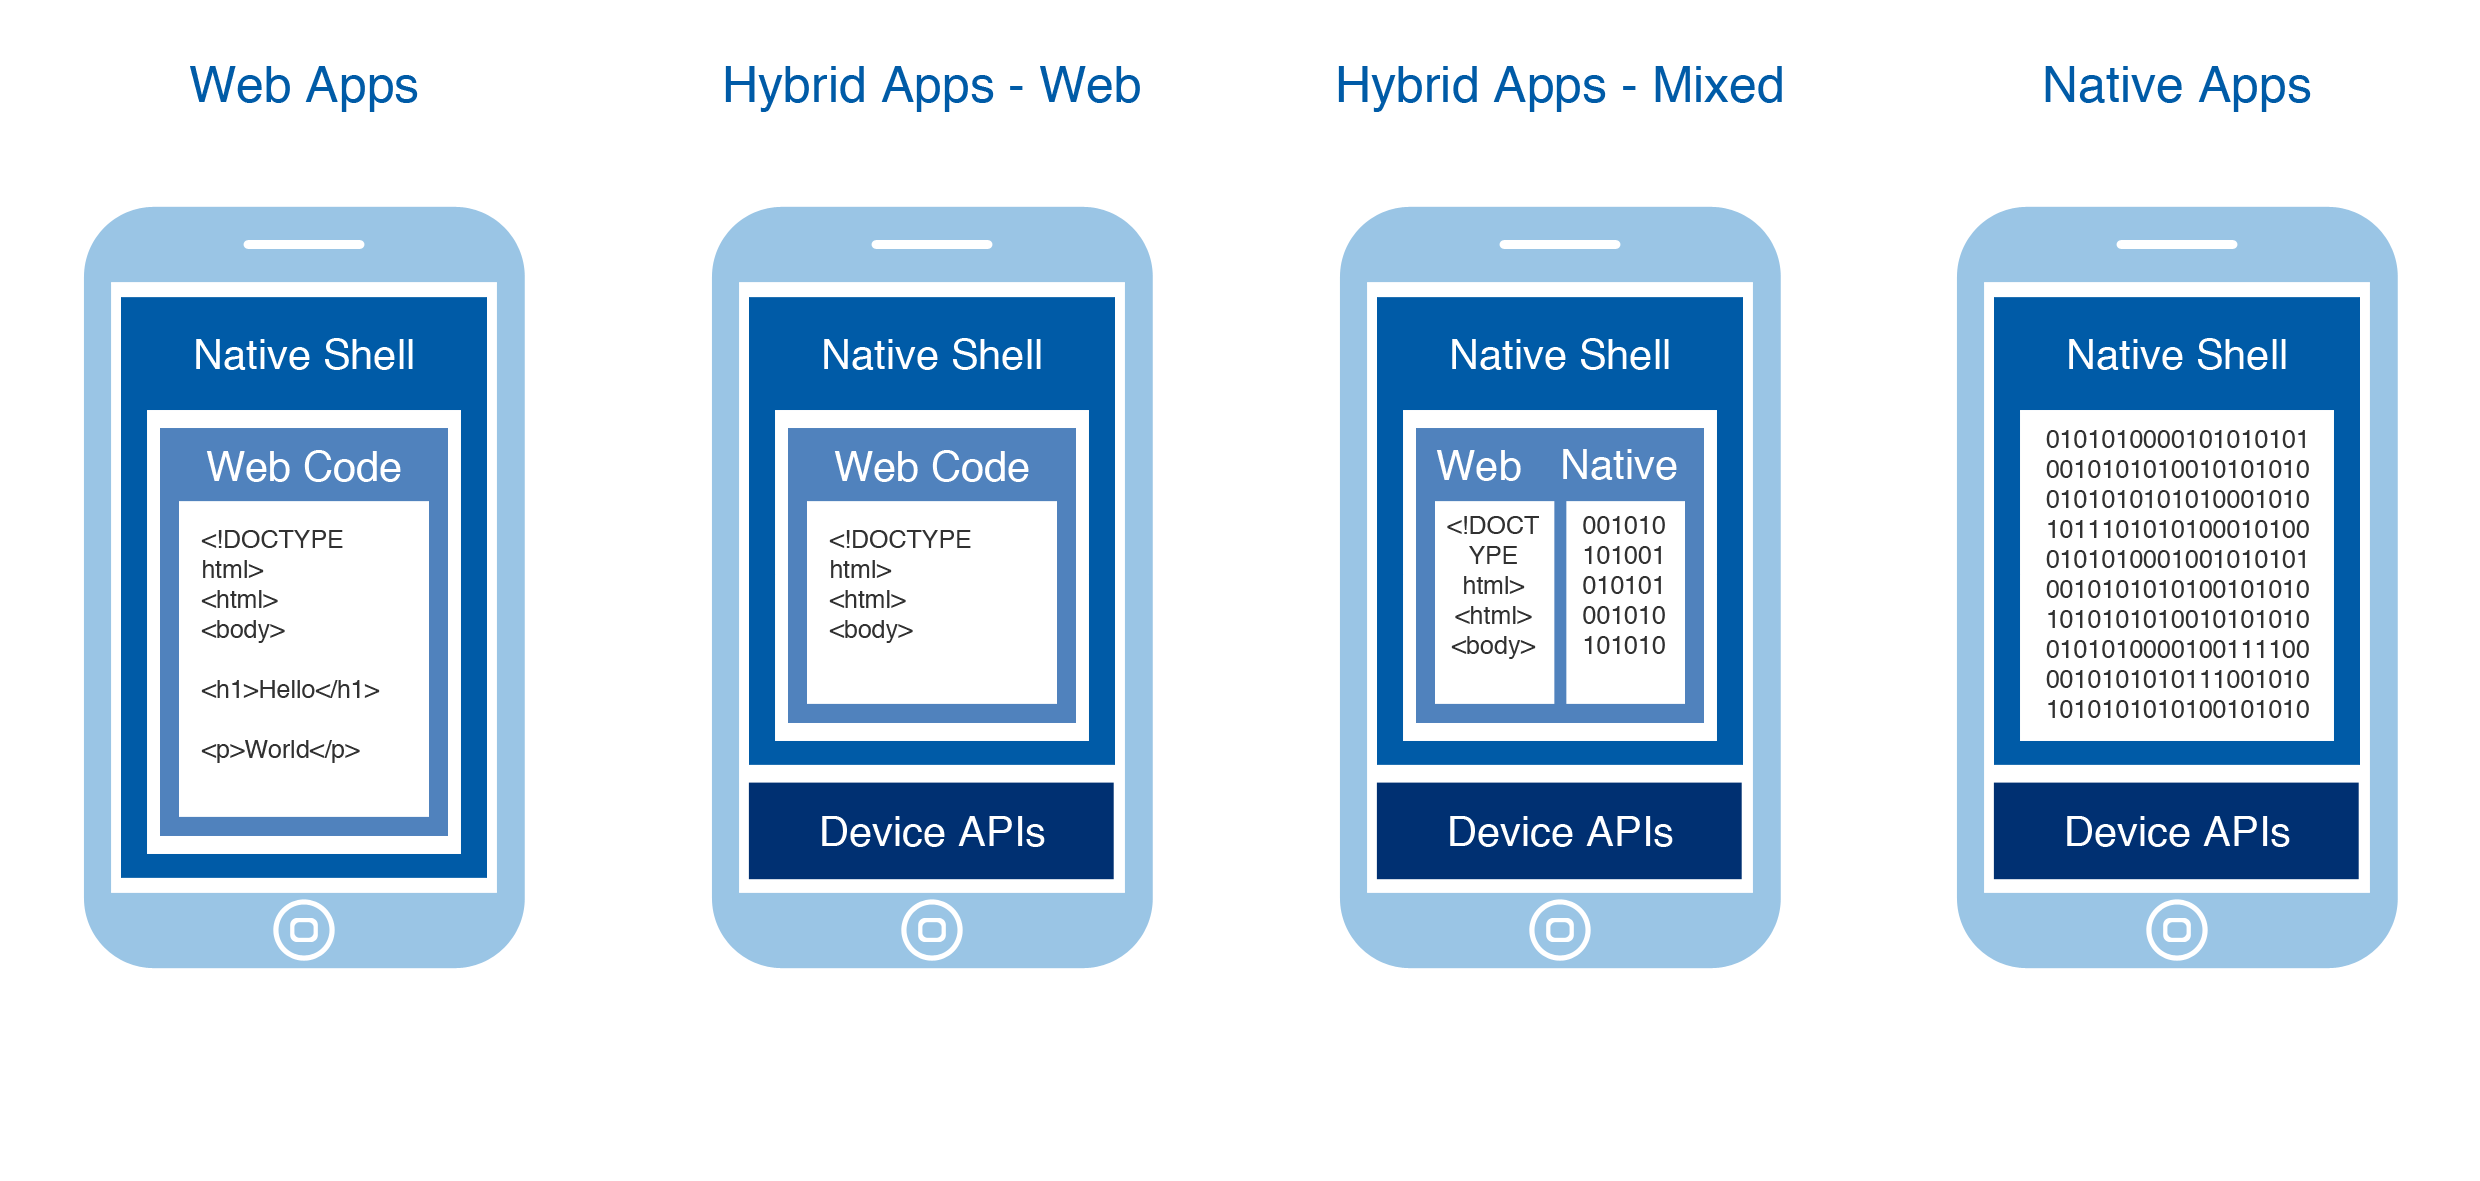
\includegraphics[scale=0.5]{images/apptypesdefined.png}\\{Different types of mobile applications\cite{IBM-Worklight2012}}\\
\end{centering}

\paragraaf{Conclusion}
A natively written mobile application provides the user with an experience immersed to that of the level of the device's operating system. This is due to two reasons:
\begin{itemize}
\item
\emph{Performance}\\
a native application is faster because it has direct access to memory and CPU
\item \emph{Looks}\\
a native application looks and feels more coherent to the device's operating system because it is able to make use the of the provided user interface elements.
\end{itemize}